\documentclass[a4paper]{article}
\usepackage[pdftex]{graphicx}
\usepackage[utf8]{inputenc}
\usepackage{enumerate}
\usepackage{siunitx}
\sisetup{locale=DE}
\usepackage{icomma}
\usepackage{amssymb}
\usepackage{tikz}
\usepackage{href-ul}
\hypersetup{
	colorlinks=true,
	linkcolor=blue,
	urlcolor=blue}
\usepackage{geometry}
\geometry{a4paper, top=15mm, left=15mm, right=15mm, bottom=15mm,
	headsep=10mm, footskip=12mm}

\begin{document}
	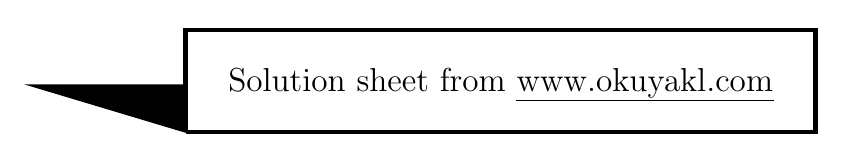
\begin{tikzpicture}(10,3)
		\draw[ultra thick](2,0) --(10,0) -- (10,1.3) --(2,1.3) -- (2,0);
		\draw[fill=black](2,0)-- (0,.6) -- (2,.6) -- (2,0);
		\node at (6,.6) {\large Solution sheet from \href{http://www.okuyakl.com}{www.okuyakl.com}};
	\end{tikzpicture}
	\vspace{0.5 cm}
	
	
	\noindent{\bf Task 1. a)}\\
	Every body has a mass. This is unchangeable and remains the same, regardless of whether the body is on the moon or on the earth. The weight is related to weight; it is a quantity that is obtained when you multiply the mass of a body by the location factor $g$ or gravitational acceleration. Thus, a body with a certain mass weighs more on Earth than on the Moon.
	\vspace{0.5 cm}
	
	\noindent{\bf Task 1. b)}\\
	The force acting on the spring is:
	$$F_F = D \cdot s = \SI{24}{\newton\over\meter} \cdot \SI{0.13}{\meter} = \SI{3.12}{\newton} \approx \SI{3.1}{\newton}$$
	The planet's location factor is:
	$$g_P = {F_F \over m} = {\SI{3,1}{\newton} \over \SI{0.15}{\kilogram}}= \SI{20,8}{\meter\over \second^2}$$
	\vspace{0.5 cm}
	
	\noindent{\bf Task 2.}\\
	The mass of the cube is (we can use centimeters and grams here):
	$$ m= \varrho \cdot V = \SI{2,7}{\gram\over {\centi\meter^3}}\cdot (\SI{4,5}{\centi\meter})^3 = \SI{246}{\gram}$$
	Its weight is equal to the spring force and therefore the elongation is $s$:
	$$D \cdot s = m \cdot g \quad \Rightarrow \quad s = {m \cdot g \over D}= {\SI{0.25}{\kilogram} \cdot \SI{9.81} {\meter\over {\second^2}} \over \SI{90}{\newton\over \meter}} = \SI{0.027}{\meter}$$
	The original spring length is:
	$$l_0 = l - s =\SI{36.0}{\centi\meter} -\SI{2.7}{\centi\meter} = \SI{33.3}{\centi\meter}$$
	\vspace{0.5 cm}
	
	\noindent {\bf task 3. a)}\\
	Hooke's law states that the spring force is proportional to the extension (=distance). To investigate this, we attach the spring, hang various weights with a weight of up to $\SI{12}{\newton}$ on it and note the elongation $s$. We enter the value pairs into a diagram. If they lie on a straight line from the origin, then Hooke's law applies to this spring.
	\vspace{0.5 cm}
	
	\noindent {\bf task 3. b)}\\
	The following applies:
	$$F=D\cdot s \qquad \Leftrightarrow \qquad s={F \over D} \qquad (*)$$
	The same force $F$ acts on both springs, so spring 1 of hardness $D_1$ stretches by $s_1$ and spring 2 of hardness $D_2$ stretches by $s_2$. The total strain is $s_{ges}=s_1+s_2$:
	$$s_{ges}=s_1+s_2= {F \over D_1}+ {F \over D_2} $$
	with inserted values we get:
	$$s_{ges}= {\SI{10}{\newton} \over\SI{250}{\newton\over {\meter^2}} }+{\SI{10}{\newton} \over \SI {500}{\newton\over \meter}}=\SI{0.060}{\meter}=\SI{6.0}{\centi \meter}$$
	The following applies to the calculation of the total spring hardness (*):
	$$D_{ges}={F\over s_{ges}}={\SI{10}{\newton}\over \SI{0.060}{\meter}}=\SI{1.7e2}{\newton \over\meter}$$
	\vspace{0.5 cm}
	
	\newpage
	\noindent{\bf Task 4.}\\
	The density of the concrete is $\varrho=\SI{2.4}{\gram\over {\centi\meter^3}}=\SI{2.4}{\kilogram\over {\deci\meter^3}}$. The volume in $\SI{}{\deci\meter^3}$ of the concrete slabs is:
	$$V=(\SI{3}{\deci\meter})^2 \cdot \SI{0.5}{\deci\meter} \cdot 150 =\SI{675}{\deci\meter^3 }$$
	This corresponds to a weight of:
	$$m=\varrho \cdot V = \SI{2,4}{\kilo\gram\over {\deci\meter^3}} \cdot\SI{675}{\deci\meter^3} = \SI{1620}{\kilo\gram}$$
	So he has to drive three times.
	\vspace{0.5 cm}
	
	\begin{center}
		\includegraphics[width=7 cm]{../../viecher/eendcomic.pdf}
		
		Here you can go back to the \href{https://www.okuyakl.de/phys/p8hukL405/ae405.pdf}{task sheet}
	\end{center}
	
\end{document}